\documentclass[UTF8,a4paper]{article}% 文档格式
\usepackage{graphicx}
\usepackage{amsmath}
\usepackage{ctex}% 输出汉字
\usepackage{times}% 英文使用Times New Roman
\usepackage[left=1.50cm,right=1.50cm,top=1.80cm,bottom=1.50cm]{geometry}% 页边距设置
\usepackage{indentfirst}% 中文首行缩进
\renewcommand{\baselinestretch}{1.5}% 定义行间距(1.5)
\usepackage{fancyhdr} %设置全文页眉、页脚的格式
\pagestyle{fancy}
\usepackage{multirow} %Table Support
\usepackage{siunitx}
\usepackage{float}
\usepackage{ctex}

\usepackage[pdfauthor={杨哲涵},
            pdftitle={基础物理实验(A1)声速测量实验报告},
            pdfcreator={Xelatex}]{hyperref}

\title{\fontsize{14pt}{27pt}\selectfont% 四号黑体
    {\heiti% 黑体 
        基础物理实验报告\\
        声速测量实验}}
\author{\fontsize{12pt}{18pt}\selectfont% 小四楷体
    {\kaishu% 楷书
    杨哲涵~~~工物22班~~~2022011105}}
\date{2023年6月1日}
\begin{document}
\maketitle
\lhead{2023年基础物理学实验A}% 页眉左边设为空
\chead{}% 页眉中间设为空
\rhead{41a}% 页眉右边设为空
\lfoot{}% 页脚左边设为空
\cfoot{\thepage}% 页脚中间显示页码
\rfoot{}% 页脚右边设为空
\section*{摘要}
波动是振动状态的传播。在无限大的空气或液体中传播的声波是纵波;固体中传播的声波,可以是纵波、横波,也可以是表面波。本实验将通过示波器等仪器测量空气中声波的频率,波长,
并利用超声波试验仪等,按照其适合的不同方法测量固体中三种波的波速,更直观地理解机械波的传播、进行与之相关的计算。
\section{实验目的}
\begin{itemize}
    \item 了解声波在空气中传播速度与气体状态参量的关系;了解声波产生和接收的原理
    \item 利用(行波近似下的)相位比较法、(驻波假设下的)振幅极值法测量空气声速,与理论值做比较
    \item 利用脉冲波信号测量固体声速,理解波在传输路径上遇到界面时的反射和透射特性,了解表面波
\end{itemize}
\section{实验仪器}
\begin{itemize}
    \item 信号发生器:Tektronix AFG1062,双通道,60 $\unit{\mega\hertz}$,采样率300$\unit{MS/s}$
    \item 示波器:Tektronix TBS1102B-EDU,双通道,100 $\unit{\mega\hertz}$,采样率2.5$\unit{MS/s}$
    \item 气体声速仪
    \item 超声波试验仪
    \item 干湿温度计
    \item 固体声速装置
    \item BNC-banana电缆
    \item BNC-BNC同轴电缆
\end{itemize}
\section{实验原理}
\subsection{理想气体中的声波}
理想气体中的声速:
$$v=\sqrt{\frac{\gamma RT}{M}}$$
其中,$\gamma=c_p/c_V$为质量热容比,$c_p$为气体的质量定压热容,$c_v$为气体的质量定容热容。
因此,声速的测定可以推算出气体的一些参量,测定温度等。

实际空气中修正后的公式为:
$$v=331.5\sqrt{1+\frac{t}{T_0}}(1+0.16\frac{rp_s}{p})\unit{m/s}$$
$$\lg p_s=10.286-\frac{1780}{237.3+t}$$
在北京,大气压$p\approx 101\unit{\kilo\pascal}$,实验中需测量相对湿度$r$,温度$t$。
\subsection{发射接收原理}
产生和接收超声波的关键元件是锆钛酸铅压电陶瓷(PZT,piezoelectric ceramic),压电陶瓷在外力作用下(如空气中的静压作用),
陶瓷体内产生与应力成线性关系的电极化强度,从而使压电陶瓷在某些相对应的端面上出现异号极化电荷,
形成电压,这一效应称为压电效应(piezoelectric effect)。在超声波的交变声压作用下,
压电陶瓷两极表面产生与声压成比例的交变电压信号,这就是声探测器的基本原理。

压电陶瓷上加上电压后,陶瓷体内会产生与电场强度成线性关系的应变,从而使陶瓷出现宏观机械形变。
这一效应称为逆压电效应。一定频率的交流电信号加在压电陶瓷上,使它产生同频机械振动,从而能发射出超声波,成为声发射器。

用于发射器与探测器的PZT材料的信号与特性依据其用途而有所不同。无论是管状或片状PZT,都有一定的共振频率,在这些频率附近能量转换效率高。
\subsection{相位比较法}
若声发射器的直径显著大于波长、声探测器的直径小于波长,则声波在探测器与发射器间的反射很少,声波可被近似为行波。

因此,在传播方向上的任何两点,如果其振动状态相同,则这两点同相位,或者说其相位差为$2\pi$的整数倍,如果振动方向完全相反,则相位差为$\pi$的奇数倍。
在示波器上观察的同时,移动探测器,相位差每隔$2\pi$或$\pi$就记录一次移动距离,即可得到$\lambda$或$\lambda/2$,这便是行波近似下的相位比较法。
\subsection{振幅极值法}
实际中,由于声探测器的尺寸并非远小于波长,在发生器与探测器间的路径上,声波既有行波的成分,也有驻波(相干叠加)的成分。
当探测器沿着入射波传播方向移动时,接收器处的声强信号会出现如图\ref{fg:amplitude}所示的准周期性变化。极大值位置之间的平均间距等于$\lambda/2$。

因此,可以通过测量极大值之间的平均间距,得到波长$\lambda$,从而得到声速$v$。
\begin{figure}[H] % 多图排版
    \centering
    \begin{minipage}[t]{0.5\linewidth}
        \centering
        \includegraphics[width=0.95\linewidth]{phase.png}
        \caption{相位比较法}
        \label{fg:phase}
    \end{minipage}%
    \begin{minipage}[t]{0.5\linewidth}
        \centering
        \includegraphics[width=0.95\linewidth]{amplitude.png}
        \caption{振幅极值法}
        \label{fg:amplitude}
    \end{minipage}
\end{figure}
\subsection{声波在固体中的传播}
超声波在介质中的传播通常有三种类型:纵波、横波或是表面波,它们的产生取决于介质可以承受何种作用力以及如何对介质激发起声波。
\paragraph{纵波波型}
当介质中质点振动方向与超声波的传播方向一致时,此超声波为纵波波型。任何固体介质当其体积发生交替变化时均能产生纵波。
\paragraph{横波波型}
当介质中质点的振动方向与超声波的传播方向相垂直时,此种超声波为横波波型。由于固体介质除了能承受体积变形外,还能承受切变变形,因此,当剪切力交替作用于固体介质时均能产生横波。横波只能在固体介质中传播。
\paragraph{薄面波波型}
沿着固体表面传播的具有纵波和横波的双重性质的波。表面波可以看成是由平行于表面的纵波和垂直于表面的横波合成,振动质点的轨迹为一椭圆,在距表面$\frac{1}{4}$波长深处振幅最强,随着深度的增加很快衰减,实际上离表面一个波长以上的地方,质点振动的振幅已经很微弱了。
\section{实验任务}
\subsection*{A.0}
实验记录室温$t$、相对湿度$r$的平均值,利用以下公式进行计算:
$$v=331.5\sqrt{1+\frac{t}{T_0}}(1+0.16\frac{rp_s}{p})\unit{m/s}$$
$$\lg p_s=10.286-\frac{1780}{237.3+t}$$
得到结果如下:
\begin{table}[H]
    \centering
    \caption{空气声速理论值}
    \label{tab:a0}
    \begin{tabular}{llll}
        \hline
        $\bar{t}(\unit{\degreeCelsius}$) & $\bar{r}$ & $p_s(\unit{\pascal})$ & $v(\unit{m/s})$ \\
        25.75                            & 54.8      & 21568.4               & 353.247         \\ \hline
    \end{tabular}
\end{table}
\subsection*{A.1}
开始本任务前,将信号发生器的OUTPUT1连接到空气声速仪的超声发射器,同时接到示波器的一个输入端CH1;空气声速仪的接收器连接到示波器的另一输入端,即CH2。

在连接时,注意将BNC阴头上的2个凸起对准BNC阳头的凹槽,插入后旋转到头(旋转约$\ang{90}$),将其拧紧;此外,空气声速仪的BNC插头被焊接在仪器上,连接时应当小心,避免用力过猛造成损坏。
\subsection*{A.2}
这一步骤确定空气中声波的频率,后续步骤中将使用该频率进行测量。

将声速仪发射器和接收器间距调整到$50\unit{mm}$左右。信号发生器设置为:正弦波,高阻,$U_{pp}=20\unit{\volt}$。将频率设置为$f=40\unit{\kilo\hertz}$。
在$0.1\unit{\kilo\hertz}$范围内调节,使得接收器在示波器上显示的信号振幅最大。随后调节接收器位置,再次使信号振幅最大。如此反复调节后,得到最大频率值为$f=40.1\unit{\kilo\hertz}$。
\subsection*{A.3}
应用实验原理中的相位比较法测量波长,即调节接收器位置的同时,记录数显卡尺的读数值,并且第一个和最后一个接收器位置相隔至少$80\unit{mm}$。

实验中测量20组数据,每次测量均取相位差为$\pi$处记录数显卡尺读数,测量结果如下:
\begin{table}[H]
    \centering
    \caption{相位比较法实验数据}
    \label{tab:a3}
    \begin{tabular}{lllllllllll}
        \hline
        序号               & 1     & 2     & 3     & 4     & 5     & 6     & 7     & 8     & 9      & 10     \\
        坐标值($\unit{mm}$) & 21.18 & 25.69 & 30.13 & 34.52 & 39    & 43.51 & 47.78 & 52.14 & 56.47  & 60.87  \\
        序号               & 11    & 12    & 13    & 14    & 15    & 16    & 17    & 18    & 19     & 20     \\
        坐标值($\unit{mm}$) & 65.15 & 69.53 & 73.94 & 78.32 & 82.75 & 87.24 & 91.69 & 96.14 & 100.67 & 104.89 \\ \hline
    \end{tabular}
\end{table}
\subsection*{A.4}
应用实验原理中的振幅极值法测量波长,即调节接收器位置的同时,记录数显卡尺的读数值,如此完成8组数据的测量,结果如下:
\begin{table}[H]
    \centering
    \caption{振幅极值法实验数据}
    \label{tab:a4}
    \begin{tabular}{llllllllll}
        \hline
        序号               & 1    & 2     & 3     & 4     & 5     & 6     & 7     & 8     & 9     \\
        坐标值($\unit{mm}$) & 7.61 & 12.17 & 16.69 & 21.23 & 25.65 & 30.12 & 34.67 & 39.08 & 43.31 \\ \hline
    \end{tabular}
\end{table}
\subsection*{A.5}
通过直线斜率拟合,即$x_j=b_0+b_{1j}$,可以得到波长$\lambda$的测量值。

其中,相位比较法的计算结果为$\lambda=8.79481203\unit{mm}$,声速$v=f\lambda=352.6719624\unit{m/s}$,与理论公式计算值符合得很好。

相位比较法的计算结果为$\lambda=8.946\unit{mm}$,声速$v=f\lambda=358.7346\unit{m/s}$,这一方法测得的声速与相位比较法相比,误差略大。
原因是在确定波形振幅极值时,由于波形的振幅变化不明显,难以准确定位波形的极值点,导致测量误差增大;此外,当发射器与接收器相距较远时,驻波成分远少于行波,因此振幅极值法的测量误差会增大。
\subsection*{B.0}
阅读使用说明和实验室提供的示波器说明后,开启超声波试验仪,将“检波”端口连到示波器CH1(超声波试验仪的其它端口空着,不要接电缆等)。将CH1的探头倍率设置为1X。利用CURSOR功能测量超声波试验仪信号源的脉冲信号周期,计算频率。
利用位置和分度调节钮,使示波器显示单个脉冲信号。改变衰减值,观察衰减器数值对脉冲波形的影响。利用MEASURE菜单“脉宽”测量等功能,分别测量记录$40\unit{\decibel}$、$60\unit{\decibel}$和$75\unit{\decibel}$时,信号的脉冲宽度。

本过程的测量结果如下:
\begin{table}[H]
    \centering
    \caption{脉冲宽度}
    \label{tab:b0}
    \begin{tabular}{cccc}
        \hline
        脉冲频率               & $40\unit{\decibel}$        & $60\unit{\decibel}$              & $75\unit{\decibel}$              \\
        $800\unit{\hertz}$ & $4.08\unit{\micro\second}$ & $843.3-853.3\unit{\nano\second}$ & $698.3-706.6\unit{\nano\second}$ \\ \hline
    \end{tabular}
\end{table}
此外,我们可以发现,衰减操作能够过滤掉部分杂波,使得所需波形清楚显示出来。
\subsection*{B.1}
设置衰减$\unit{\dB}$数为$75\unit{\dB}$,利用直探头测量试样铝块中纵波声速$u_l$及钻孔缺陷深度$h$,并计算不确定度。

已知数据为:试样铝块高度$H=R_2=60.10\unit{mm}$,$R_1=30.00\unit{mm}$,
它们的不确定度$U_H=U_{R_1}=U_{R_2}=0.02\unit{mm}$,密度$\rho=2700\unit{kg/m^3}$,示波器时间测量的不确定度$U_t$近似取时间轴$M$值的$\frac{1}{10}$。

可以通过波形确定探头好快,即进行接线操作的同时观察示波器,会发现BNC接头连接后示波器上出现波形变化,这就证明探头正常工作。
在测量时,由于探头本身对波信号的延迟,使用脉冲信号的一级回波距发射延迟$\Delta t$进行计算并不是最优选择,因此可以通过将一、二级回波到达时间相减滤去探头的影响。

声速及孔深的计算公式与不确定度估计由以下式子给出:
$$u_l=\frac{2H}{\Delta t_1},~U_{u_l}=\frac{2}{\Delta t_1}\sqrt{U_H^2+\frac{H^2}{\Delta t_1^2}U_{\Delta t_1}^2}$$
$$h=\frac{u_l\Delta t_2}{2},~U_h=\frac{1}{2}\sqrt{(\Delta t_2 U_{u_l})^2+(vU_{\Delta t_2})^2}$$
测量及带入数据的计算结果为:
\begin{table}[H]
    \centering
    \caption{B.1测量及计算结果}
    \label{tab:b1}
    \begin{tabular}{cccccc}
        \hline
        一二级全高度回波$\Delta t_1$       & $U_{\Delta t_1}$          & 一二级孔深回波$\Delta t_2$       & $U_{\Delta t_2}$          & $u_l$                        & 孔深                        \\
        $19.2\unit{\micro\second}$ & $0.5\unit{\micro\second}$ & $4.0\unit{\micro\second}$ & $0.5\unit{\micro\second}$ & $(6.26 \pm 0.16)\unit{km/s}$ & $(12.5 \pm 1.6)\unit{mm}$ \\ \hline
    \end{tabular}
\end{table}
\begin{figure}[H] % 多图排版
    \centering
    \begin{minipage}[t]{0.5\linewidth}
        \centering
        \includegraphics[width=0.95\linewidth]{B1-1.jpg}
        \caption{一二级全高度回波$\Delta t_1$}
        \label{fg:b1-1}
    \end{minipage}%
    \begin{minipage}[t]{0.5\linewidth}
        \centering
        \includegraphics[width=0.95\linewidth]{B1-2.jpg}
        \caption{一二级孔深回波$\Delta t_2$}
        \label{fg:b1-2}
    \end{minipage}
\end{figure}
\subsection*{B.2}
设置衰减$\unit{\dB}$数为$60\unit{\dB}$,利用$\ang{45}$斜探头对试样铝块中横波声速$u_s$进行测量。
\begin{figure}[H] % 多图排版
    \centering
    \begin{minipage}[t]{0.5\linewidth}
        \centering
        \includegraphics[width=0.95\linewidth]{B2-1.png}
        \caption{测量原理}
        \label{fg:b2-1}
    \end{minipage}%
    \begin{minipage}[t]{0.5\linewidth}
        \centering
        \includegraphics[width=0.95\linewidth]{B2-2.jpg}
        \caption{扇环回波$\Delta t$}
        \label{fg:b2-2}
    \end{minipage}
\end{figure}
测量原理为$\ang{45}$斜探头放置在图\ref{fg:b2-1}中(2)位置,从探测器发出的波会经过$R_1$与$R_2$反射回探头,再结合时间差即可得到声速,即:
$$u_s=\frac{2(R_2-R_1)}{\Delta t}$$
测量及带入数据的计算结果为:
\begin{table}[H]
    \centering
    \caption{B.2测量及计算结果}
    \label{tab:b2}
    \begin{tabular}{cccc}
        \hline
        $R_1$           & $R_2$           & $\Delta t$                 & $u_s$              \\
        $30.0\unit{mm}$ & $60.1\unit{mm}$ & $19.4\unit{\micro\second}$ & $3103.1\unit{m/s}$ \\ \hline
    \end{tabular}
\end{table}
\subsection*{B.3}
利用可变角探头,观察表面波的产生,测量表面波声速$u_R$。

在进行实验时,设置衰减$\unit{\dB}$数为推荐值$40\unit{\dB}$,并令探头入射角为$\ang{65}$,沾湿探头表面后接触试样铝块表面,可以在示波器上观察到表面波回波信号。

我们可以观察到,由于表面波衰减较快,波器上的回波信号振幅较弱。此外,由于表面波沿着固体表面的传播特性,用手掌按压铝块表面,可以看到回波信号消失;抬起手掌后,信号再次出现,这就证明了该信号确为表面波。此外,将水滴($1\unit{ml}$以上)滴在试样铝块表面,
可以发现回波信号同样消失了,吸干水滴后,回波信号同样会再次恢复。

为了测量表面波声速,我们可以在试样铝块上,沿着平行铝块边界方向移动探头,记录下探头移动的距离,结合移动后回波的时间差,即可得到波速:
$$u=\frac{2(x_1-x_2)}{\Delta t}$$
\begin{table}[H]
    \centering
    \caption{B.3测量及计算结果}
    \label{tab:b3}
    \begin{tabular}{cccc}
        \hline
        $x_1$           & $x_2$           & $\Delta t$                 & $u_R$              \\
        $80.6\unit{mm}$ & $33.5\unit{mm}$ & $32.4\unit{\micro\second}$ & $2907.4\unit{m/s}$ \\ \hline
    \end{tabular}
\end{table}
\begin{figure}[H] % 多图排版
    \centering
    \begin{minipage}[t]{0.5\linewidth}
        \centering
        \includegraphics[width=0.95\linewidth]{B3-1.jpg}
        \caption{$x_1$处光标}
        \label{fg:b3-1}
    \end{minipage}%
    \begin{minipage}[t]{0.5\linewidth}
        \centering
        \includegraphics[width=0.95\linewidth]{B3-2.jpg}
        \caption{$x_2$处光标}
        \label{fg:b3-2}
    \end{minipage}
\end{figure}
\subsection*{B.4}
根据实验B.1以及B.2,使用如下公式可计算实验所用试样的弹性模量和泊松比。
$$E=\frac{\rho u_s^2(3T^2-4)}{T^2-1}$$
$$\sigma=\frac{T^2-2}{2(T^2-1)}$$
其中$T=\frac{u_l}{u_s}$,$\rho$为材料密度。
代入先前所测数据为:
\begin{table}[H]
    \centering
    \caption{B.4计算结果}
    \label{tab:b4}
    \begin{tabular}{ccccc}
        \hline
        $u_l$               & $u_s$              & $\rho$              & $E$                & $\sigma$ \\
        $6260.42\unit{m/s}$ & $3103.1\unit{m/s}$ & $2700\unit{kg/m^3}$ & $69.53\unit{\GPa}$ & 0.3371   \\ \hline
    \end{tabular}
\end{table}
查阅资料可得,硬铝合金的弹性模量通常为$70\unit{\GPa}$,泊松比通常为0.3,这与实验符合得较好。
\section{讨论}
\paragraph{可变角探头}
可变角探头的推荐入射角为$\ang{65}$,这与入射纵波在介质界面上的反射与折射有关,根据Fresnel折射定律,有:
$$\frac{\sin\theta}{u_{1l}}=\frac{\sin\beta_l}{u_{2l}}=\frac{\sin\beta_s}{u_{2s}}$$
其中折射角与入射角在图\ref{fg:dis-1}中标出。可以看出,若$\sin\theta>\frac{u_{1l}}{u_{2s}}$且$\sin\theta>\frac{u_{1l}}{u_{2l}}$,则介质中既无纵波折射,也无横波折射,这种情况将会产生表面波。

因此,在实验中入射角的调节需满足以上条件。已知探头嵌在纵波声速为$u=2680\unit{m/s}$的有机玻璃中,硬铝合金的纵波声速与横波声速分别为$6260\unit{m/s}$,$3103\unit{m/s}$,
可计算得出,满足条件的$\theta\geq\ang{59;43}$才可出现表面波。实验中选用$\ang{65}$是为了保证纵波成分与横波成分均不出现,且要避免大角度入射,以免接收到回波的幅度过小。

此外,在测量横波时使用$\ang{45}$斜探头也是这一原理,即要求$\ang{25;20}\geq\theta\geq\ang{59;43}$才能在硬铝合金介质中激发横波。
\begin{figure}[H] % 多图排版
    \centering
    \begin{minipage}[t]{0.5\linewidth}
        \centering
        \includegraphics[width=0.95\linewidth]{fresnel.png}
        \caption{入射纵波在介质界面上的反射与折射}
        \label{fg:dis-1}
    \end{minipage}%
    \begin{minipage}[t]{0.5\linewidth}
        \centering
        \includegraphics[width=0.95\linewidth]{r-t.png}
        \caption{机械波在界面处的反射与透射}
        \label{fg:dis-2}
    \end{minipage}
\end{figure}
\paragraph{水膜在实验中的作用}
在实验操作中,为了使探头接收到的回波清晰可见,可以在硬铝合金表面滴几滴水滴,使得探头接触表面时形成水膜。这是由于机械波传播的阻抗性质。

机械波传播介质的特性阻抗为$Z=\rho u$,$\rho$为介质密度,$u$为介质中的波速。且垂直入射情况下机械波在界面处的能流的透射系数为$T=I_2/I_1=4Z_1Z_2/(Z_1+Z_2)^2$。从而$Z_1$与$Z_2$大致相等时透射系数最大,
否则相当部分的能流会被反射回去。由于实际中探头与介质表面往往存在缝隙,因此机械波在其中传播时经历了“探头-空气-铝块”两层界面。由于空气密度与声速显著地低,空气与二者的阻抗相差很大,使得能流透射系数较低。
如能形成一层水膜,则界面间介质的阻抗更相近,可以提高透射系数。
\appendix
\section{原始数据}
\begin{figure}[H] % 多图排版
    \centering
    \begin{minipage}[t]{0.5\linewidth}
        \centering
        \includegraphics[width=0.95\linewidth]{1.jpg}
        \caption{A.0-A.4}
    \end{minipage}%
    \begin{minipage}[t]{0.5\linewidth}
        \centering
        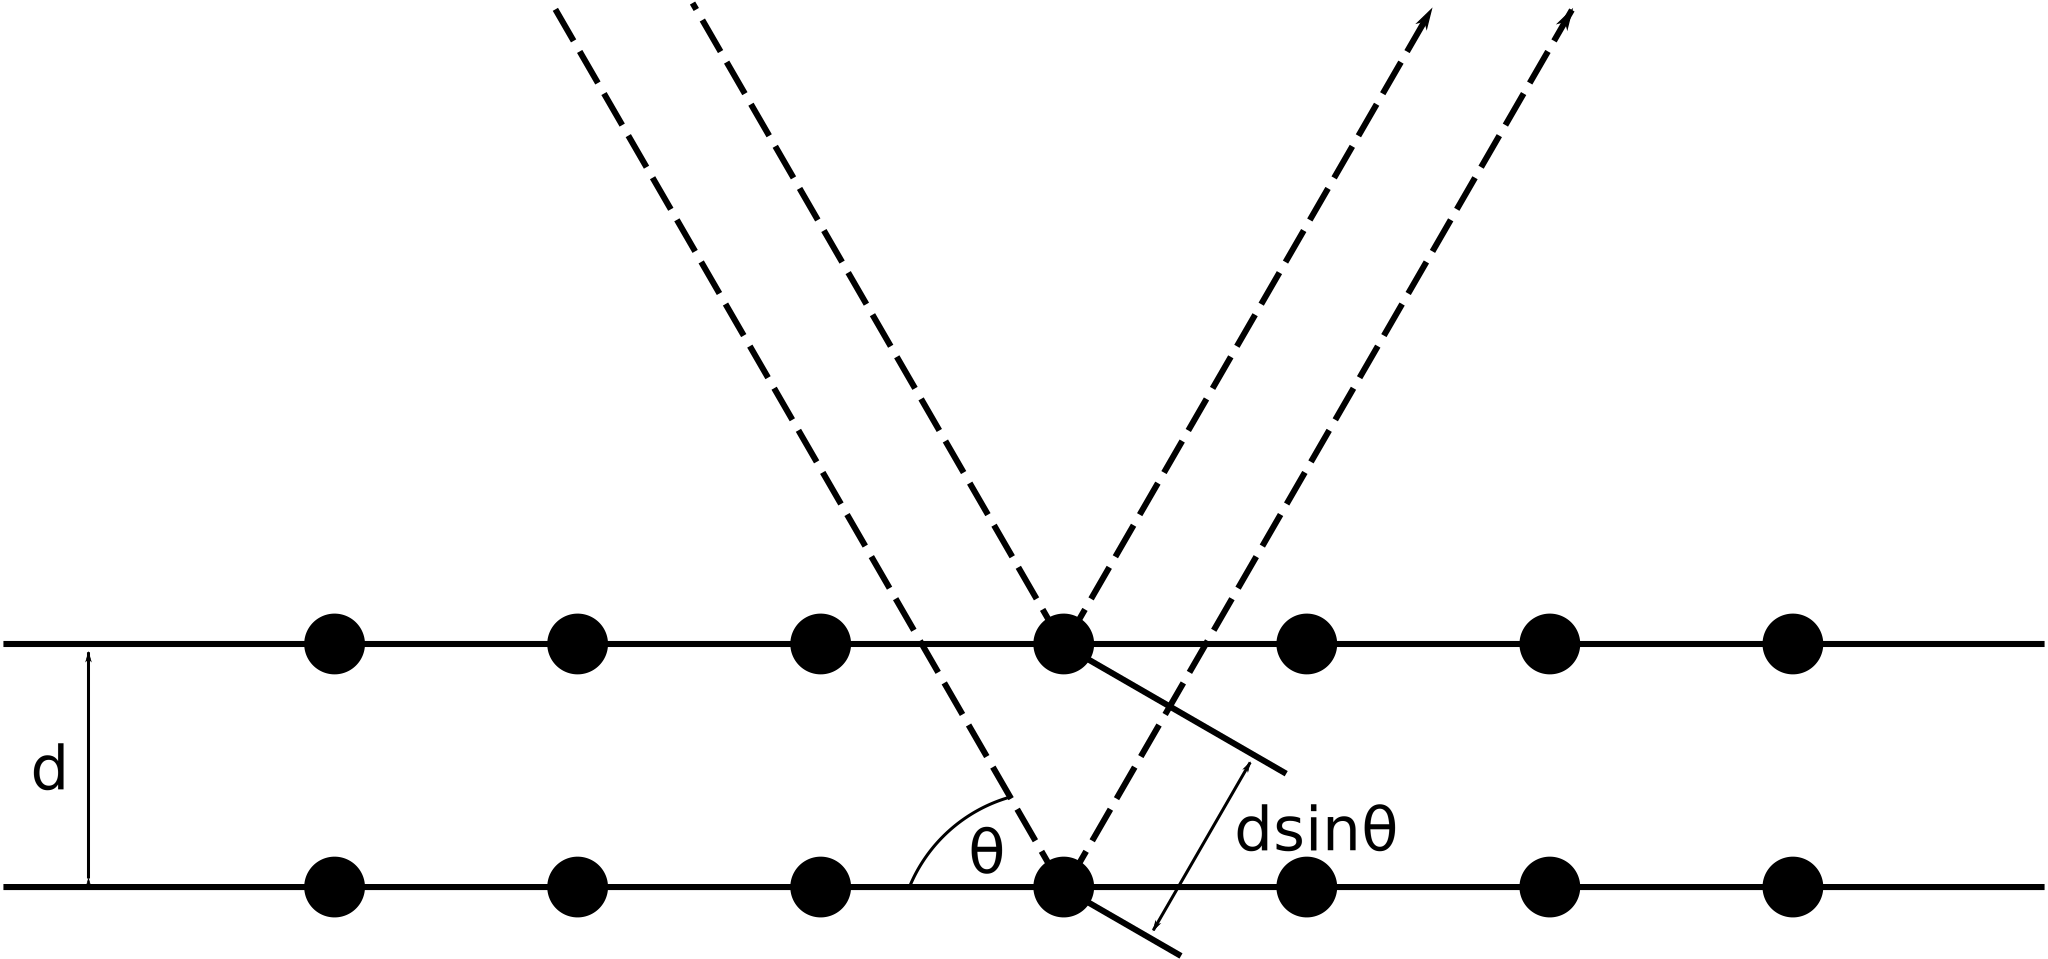
\includegraphics[width=0.95\linewidth]{2.jpg}
        \caption{B.0-B.3}
    \end{minipage}
\end{figure}
\end{document}